%% Draft outline
\section{Summary of Htrack}
\section{Model fitting with Convolution surfaces}
\section{Tracking with Convolution surfaces}
\section{Results}

\subsection{Explaining tracking parameters}
\begin{figure}[h!] 
	\centering
	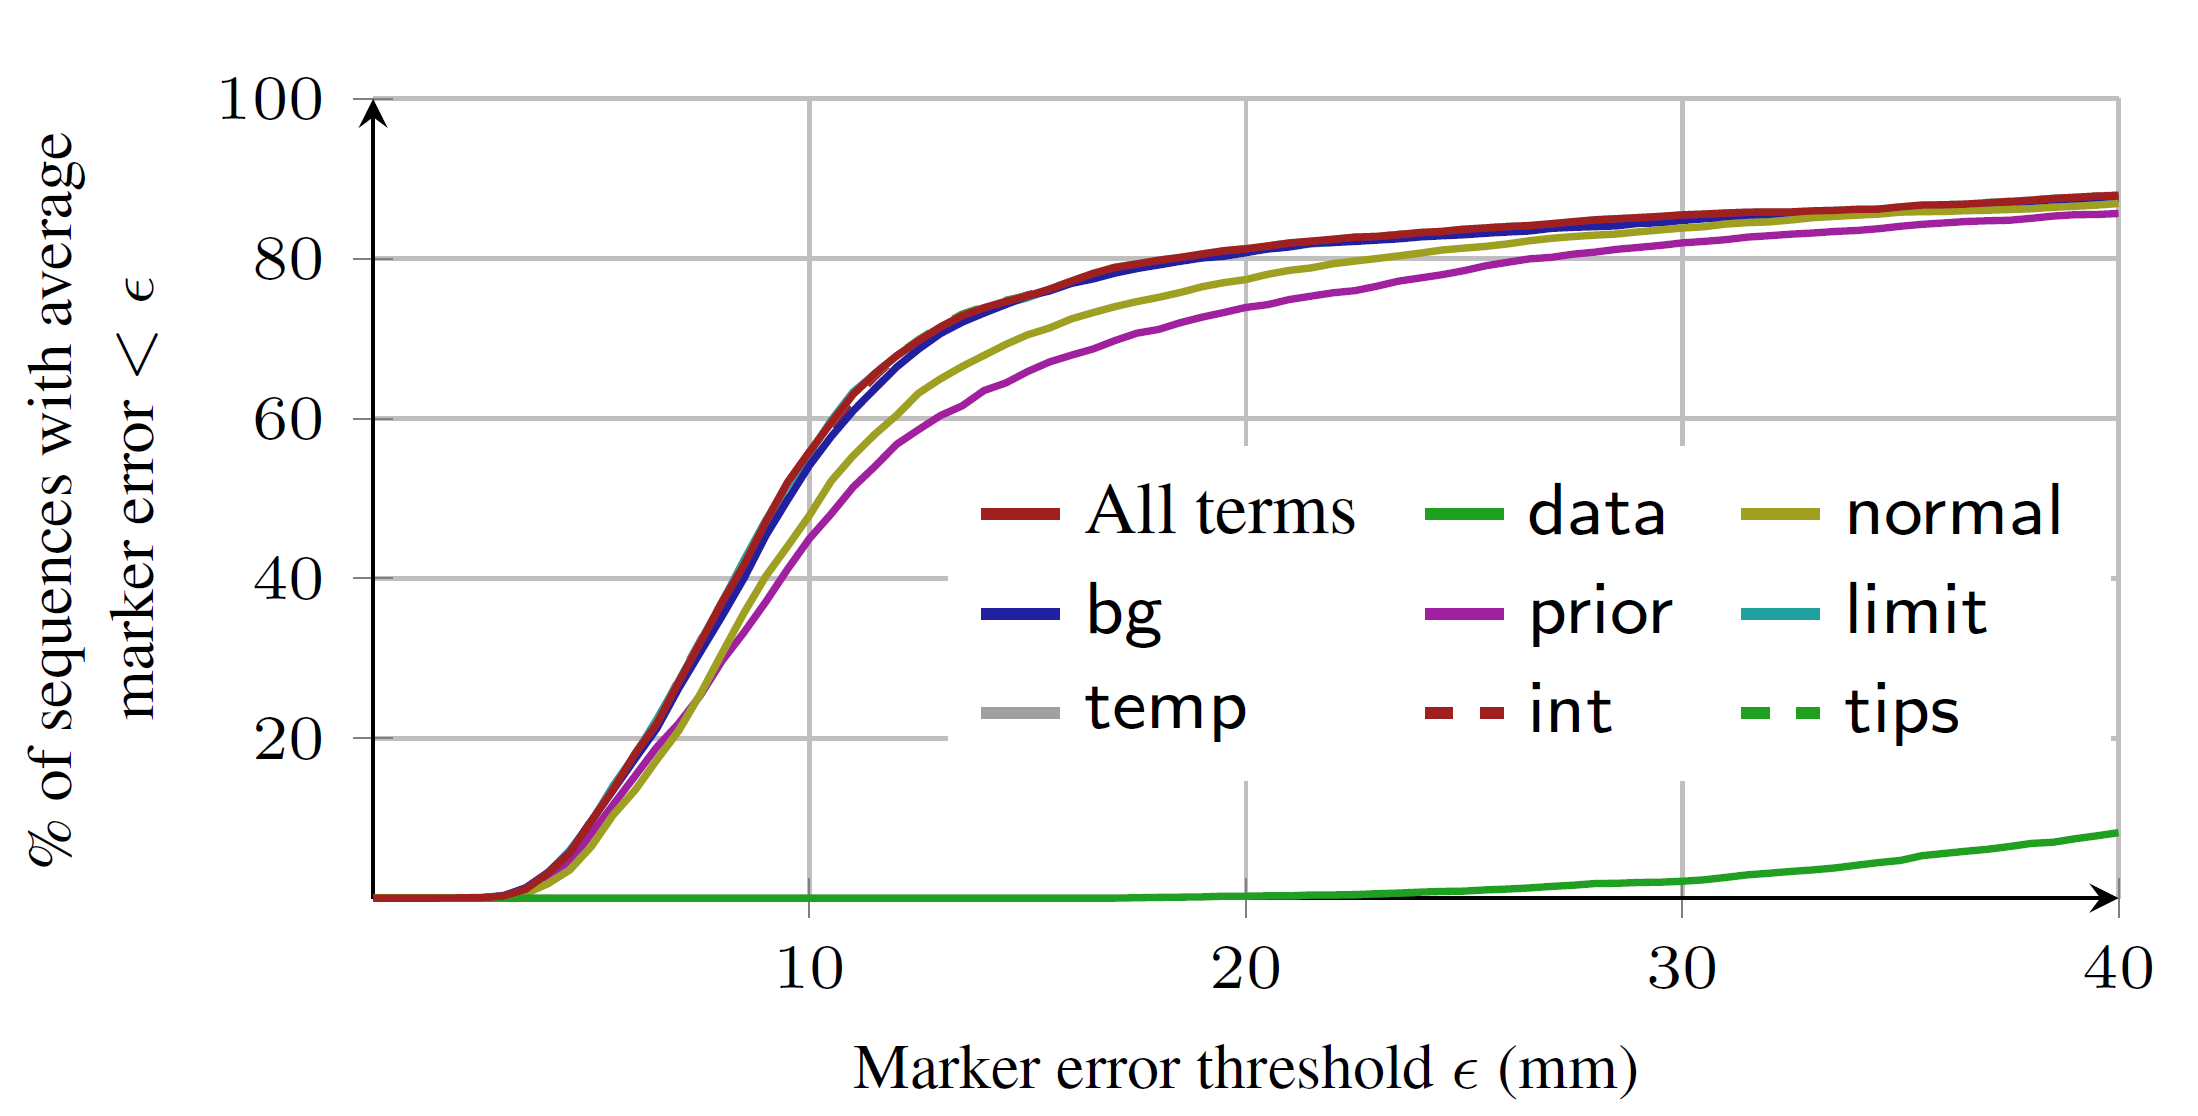
\includegraphics[width=0.5\textwidth]{fig/draft/draft_explaining_parameters}
	\caption{The performance could be measured either using online quality metrics or by generating synthetic data and adding noise}
	\label{fig:modeling}
\end{figure}

\subsection{Quantitative comparison (with Htrack)}
\begin{figure}[h!] 
	\centering
	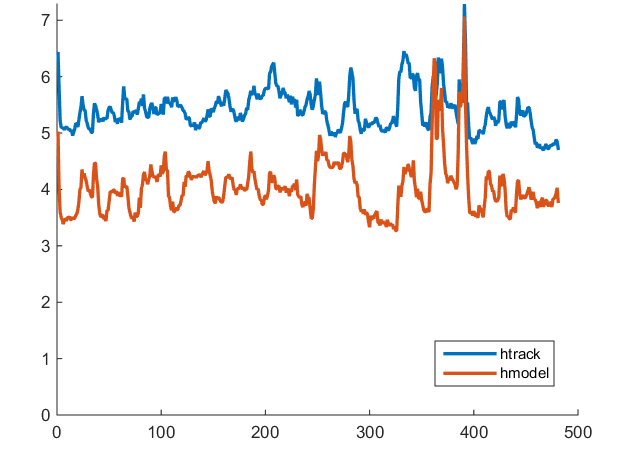
\includegraphics[width=0.5\textwidth]{fig/draft/draft_pull_error}
	\caption{Average data-model distance}
	\label{fig:modeling}
\end{figure}
\begin{figure}[h!] 
	\centering
	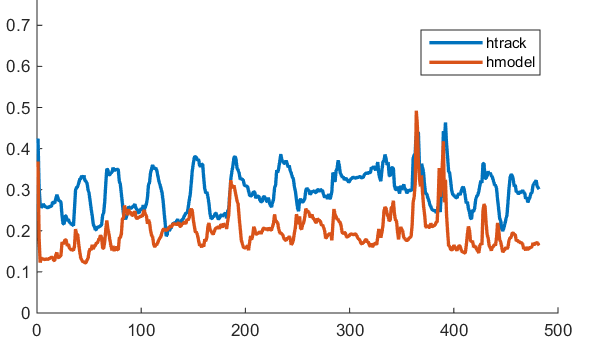
\includegraphics[width=0.5\textwidth]{fig/draft/draft_push_error}
	\caption{Silhouettes overlap}
	\label{fig:modeling}
\end{figure}
\begin{figure}[h!] 
	\centering
	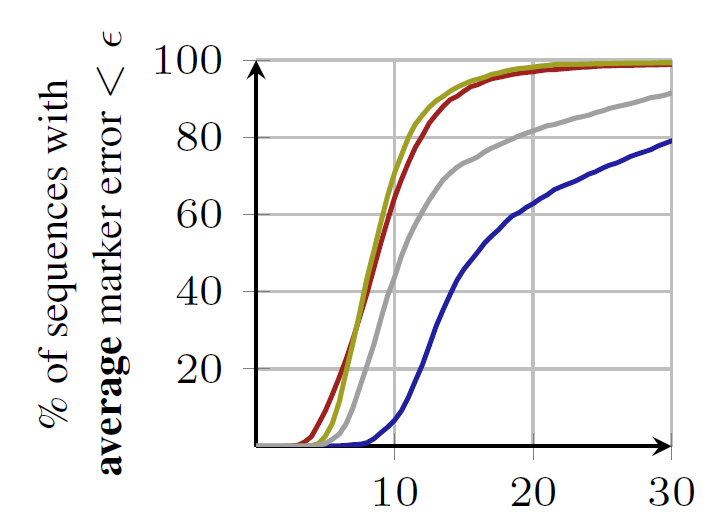
\includegraphics[width=0.5\textwidth]{fig/draft/draft_hmodel_htrack_comparison}
	\caption{Comparison on a dataset, not clear if this is possible to generate}
	\label{fig:modeling}
\end{figure}

\subsection{Hand motion classification}
\begin{figure}[h!] 
	\centering
	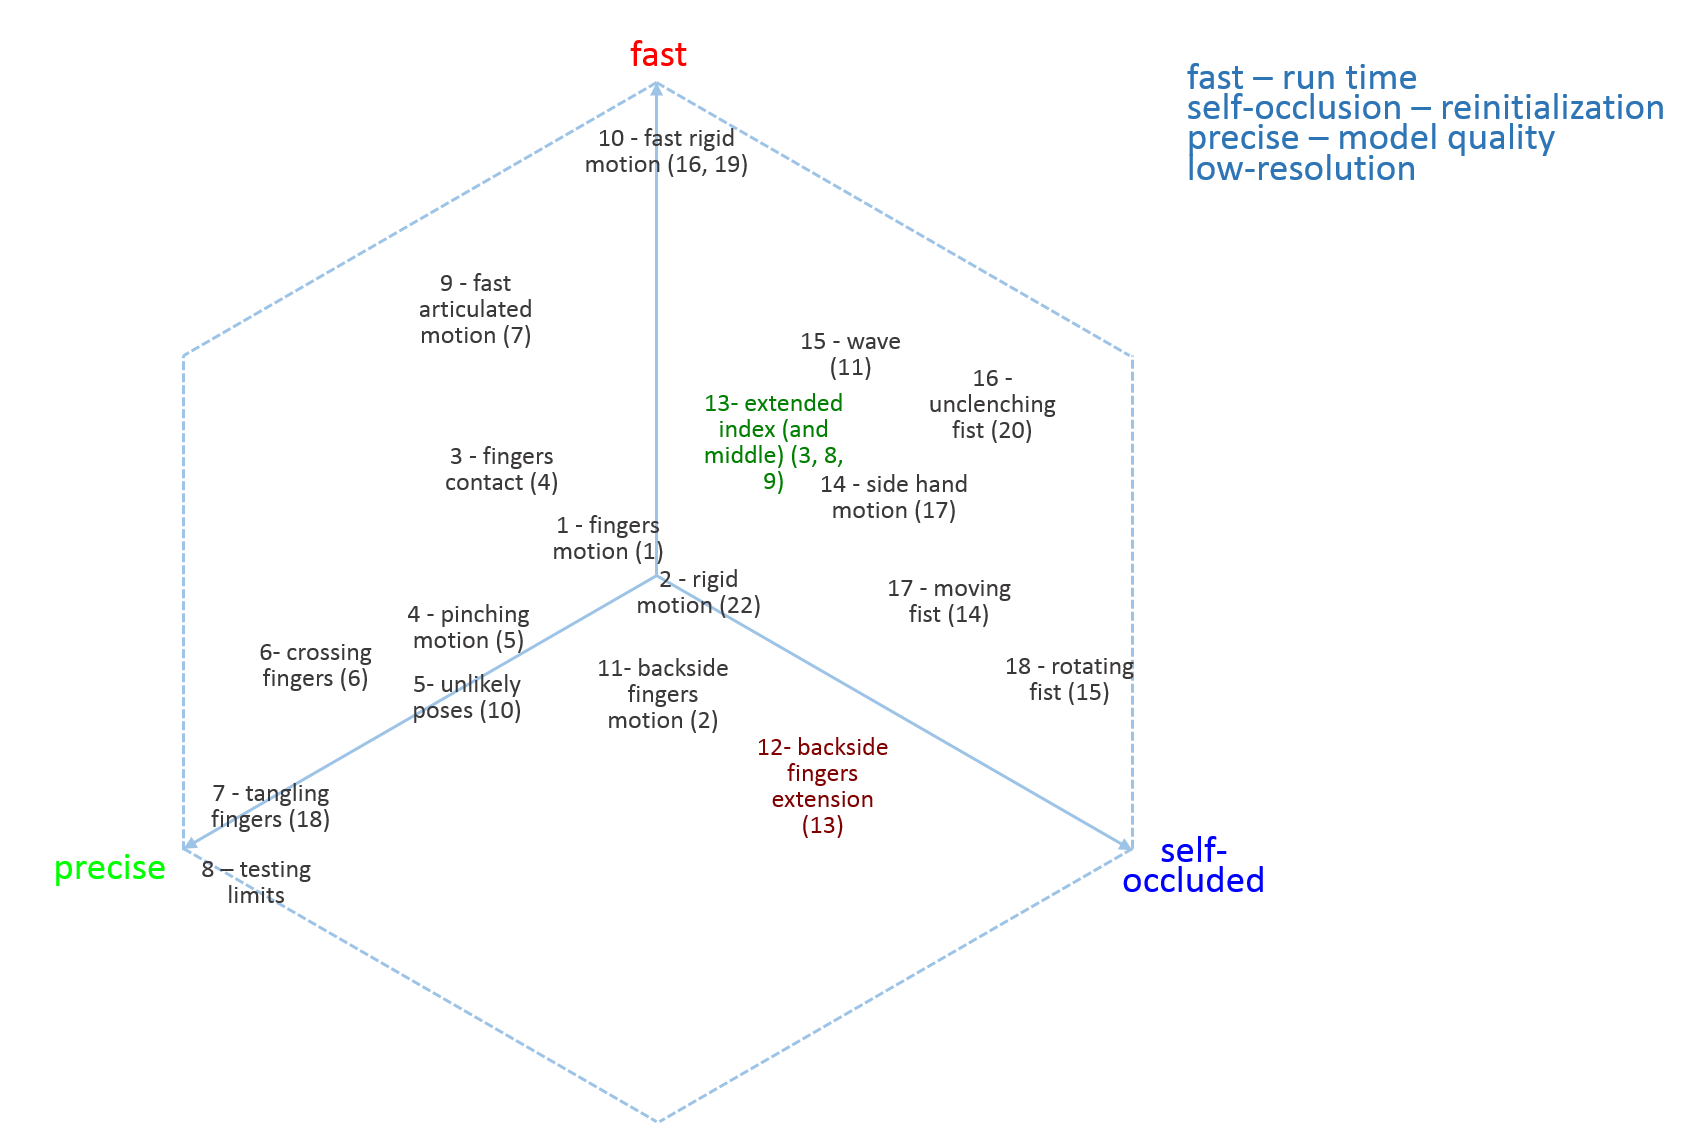
\includegraphics[width=0.5\textwidth]{fig/draft/draft_hand_motion_classification}
	\caption{Axis of motion complexity}
	\label{fig:modeling}
\end{figure}
\subsection{Qualitative comparison (with previous works)}
\begin{figure}[h!] 
	\centering
	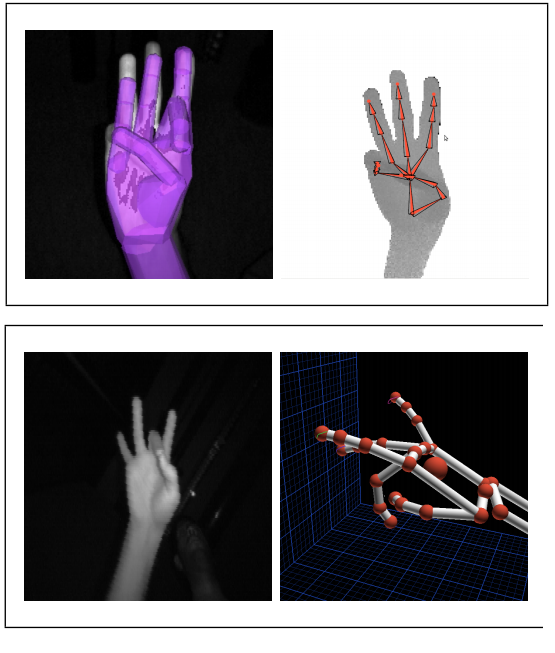
\includegraphics[width=0.5\textwidth]{fig/draft/draft_visual_comparison}
	\caption{Visual comparison}
	\label{fig:modeling}
\end{figure}